\chapter{The Wu Experiment}
\label{cha:wu_exp}

% \section{Theoretical Background}\label{sec:background}

% In order to understand the Wu experiment entirely, it is necessary to discuss the theory behind it first.
The Wu experiment focuses on the parity transformation $\hat P$, charge conjugation transformation $\hat C$ and its combination $\hat C\hat P$.
In physics, parity describes the symmetry of spatial coordinates.
% A given point in space-time would change its sign in all spatial coordinates under a parity transformation, leaving the time unchanged. %, under a parity transformation, thus the initial point would change into $(t, -x, -y, -z)$.
A given point $(t, \vec x)$ would transform to $(t, -\vec x)$ under $\hat P$.
Classical physics is invariant under parity transformation thus conserving parity. %, meaning that all laws of physics are the same in both the untransformed and transformed system and that furthermore no system is better than the other.
% This principle is known as parity conservation.
% Due to this conservation, it is not possible to confirm if a process happens in a system before or after a parity transformation.
The intrinsic parity of a particle is calculated via the spin $l$ by $ \hat P=(-1)^l$. %\inlineequation[eq:intrinsicParity]{\hat P=(-1)^l}. %$\hat P=(-1)^l$.
% \begin{align}
%     \hat P=(-1)^l.
%     \label{eq:intrinsicParity}
% \end{align}
% The parity of an ensemble of particles is a combination of the spatial parity of the system and the intrinsic parity of the different particles.
% Vectors that do not change when being transformed are called axial vectors while those that do are just called vectors. 
% An example of this is the angular momentum $\vec L$ which is invariant while the radius $\vec r$ and the momentum $\vec p$ change under transformation. \newline
As classical physics is invariant under the change of sign in spatial coordinates, it is also invariant under the change of sign of electric charges.
% If, for example, the electric charge that produces a magnetic field will change its sign, then the magnetic field itself will also change its sign thus leaving the process invariant.
In elementary particle physics, the change of sign of electric charges is called charge conjugation transformation $\hat C$ converting particles into anti-particles and vice versa, $\hat C \ket{e} = \ket{\bar e}$.
% As the only difference between particles and anti-particles is the electrical charge of the particles, a charge conjugation transformation converts particles into anti-particles and vice versa, $\hat C \ket{e} = \ket{\bar e}$.
% \begin{align}
%     \hat C \ket{e} = \ket{\bar e}.
% \end{align}
By 1957, significant discoveries in particle physics had already taken place, such as $e^\pm,\ \nu_e,\ \mu, p, \gamma,\ \pi$ and $K$.
% The most significant particles known at the time of the Wu experiment are the electron, the proton, the photon, the muon, the pion and the electron neutrino \cite{Ward:2665175}.
Parity conservation was evident for the electromagnetic (EM), the strong and the gravitational interaction, but there was no experimental evidence for parity conservation in the weak interaction \cite{CaseStudies}.
For most physicists, it seemed self-evident that parity is conserved in the weak interaction as well.
% The reason for their doubt was the $\theta-\tau$-puzzle, which described the problem of two particles having the same mass, electric charge and lifetime, but a different intrinsic parity and different decay processes.
% While the theta-meson decayed into two pions, the tau-meson decayed into three.
% Their respective intrinsic parity is $\hat P(\Theta^+)=+1$ and $\hat P(\tau^+)=-1$. %calculated via equation (\ref{eq:intrinsicParity}) is the following
% \begin{align}
%     \label{eq:calculatedParity}
%     \hat P(\Theta^+) &= (-1)\cdot(-1)\cdot (-1)^{\text{Spin}=0}=+1, \\
%     \hat P(\tau^+) &= (-1)^3\cdot (-1)^{\text{Spin}=0}=-1.
% \end{align}
% If parity is not conserved, the two particles could be two states of the same particle and the $\theta-\tau$-puzzle would be solved.
% They thus proposed many experiments to test this \cite{PhysRev.104.254}.
% The first to carry out such an experiment was Chien-Shiung Wu (1912-1997), a Chinese-American physicist who worked on the Manhattan Project at Columbia University in 1944 where she helped to develop a process to separate uranium.
% She was later offered a position at Columbia to investigate the $\beta$-decay and became one of the first to confirm Fermi's theory of the $\beta$-decay.
% It was in 1956 when she was approached by Lee and Yang for her expertise in $\beta$-decay and to carry out one of the experiments proposed earlier by them.
In 1956 however, Tsung-Dao Lee (*1926) and Chen Ning Yang (*1922) considered the conservation of $\hat P$ in the weak interaction and proposed different experiments to test it  \cite{PhysRev.104.254}.
\begin{wrapfigure}{r}{5.5cm}
    \centering
    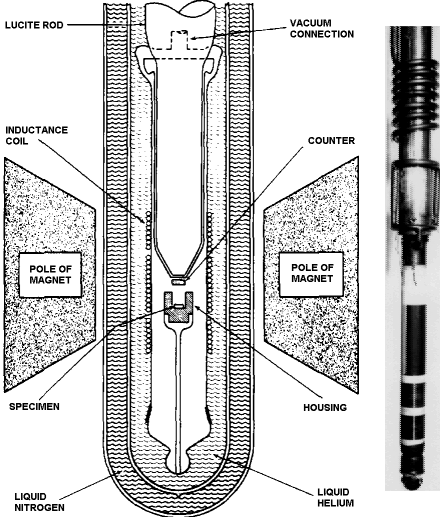
\includegraphics[width=0.35\textwidth]{figs/setup.png}
    \caption{Schematic illustration and photograph of the apparatus \cite{NIST}.}
    \label{fig:setup}
\end{wrapfigure}
The first to carry out such an experiment was Chien-Shiung Wu (1912-1997) when she was approached by Lee and Yang for her expertise in $\beta$-decay in 1956.
The experiment was based on the decay of Cobalt via $\cobalt\rightarrow \nickel+e^-+2\gamma+\bar\nu_e$.
Cobalt has a spin of 5 and was used because it decays via a $\beta$-decay into excited nickel with a spin of 4 meaning that the particles have to have the same spin direction.
Due to the polarization of the nucleus, the electrons are emitted either up- or downwards.
% The principle was to measure the angle $\vartheta$ between $e^-$ and the $\cobalt$-nucleus which is polarized so that the electrons are emitted either up- or downwards.
The emission of the electrons is invariant under parity transformation if it is conserved in the weak interaction and vice versa.
A cerium magnesium nitrate (CMN)-crystal with a small layer of cobalt was used as the specimen and placed inside a housing necessary to hold the polarization \cite{CaseStudies} which was caused by a magnetic field.
% The housing is necessary to uphold the polarization because the heat would otherwise reach the CMN and cause a rise in temperature as first tests of the experiments have shown \cite{CaseStudies}.
% A magnet was used to cool the specimen to $\approx \SI{0.003}{\kelvin}$ via adiabatic demagnetization where an inductance coil served as the thermometer.
A schematic illustration with a photograph of the used apparatus is shown in figure \ref{fig:setup}.
\begin{wrapfigure}{L}{5.5cm}
    \centering
    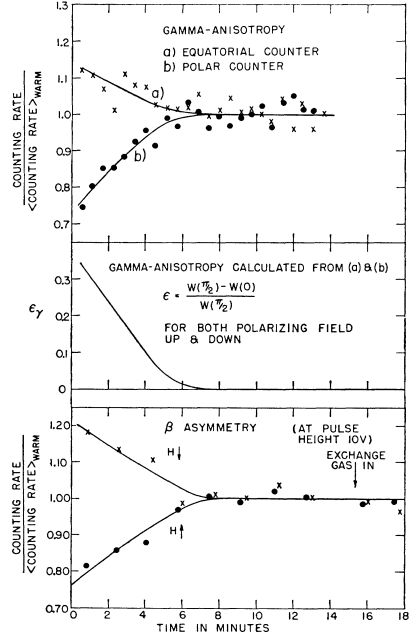
\includegraphics[width=0.4\textwidth]{figs/resultsWu.png}
    \caption{Measured results showing the gamma anisotropy and electron asymmetry for a polarizing magnetic field pointing up and down \cite{PhysRev.105.1413}.}
    \label{fig:resultsWu}
\end{wrapfigure}
An anthracene crystal was used as a scintillation counter and placed inside the lucite rod.
Sodium iodide gamma-scintillation counters were installed externally to measure the $\gamma$.
% After the first attempts in which the housing was installed to shield the CMN from heat and to keep the polarization lasting longer and after the housing "came tumbling down" \cite{Wu:2008zzm} fine nylon threats were used to bind the crystals together, the apparatus was complete and the experiment worked.
% To test for parity nonconservation the nucleus was polarized causing the electrons to be emitted up or down.
If the magnetic field is repolarized, the electron emission rates will stay the same if parity is conserved. % and vice versa.
The $\gamma$-scintillation counters were used to measure the state of the polarization because the originally isotropic emission changes under parity transformation to an oval anisotropy as this is an electromagnetic process that conserves parity \cite{CaseStudies}.
The experimental results are shown in figure \ref{fig:resultsWu}.
The measured electron rates show a clear dependence on the polarization direction. % of the magnetic field with higher counting rates with the polarizing field pointing down than up.
This asymmetry in the emission of electrons is violating parity conservation proofing \cite{PhysRev.105.1413}.
By comparing the $\gamma$ and $\beta$ emissions for similarities, it can be seen that the $\beta$ asymmetry reduces when the $\gamma$ anisotropy reduces indicating that it is not due to misalignment of the apparatus.
Further systematic checks have been made showing no dependence on systematic uncertainties \cite{CaseStudies}.
Parity nonconservation in the weak interaction also implies the violation of charge conjugation assuming its combination is conserved.

The measured asymmetry was quantified by comparing the $\beta$ asymmetry with the $\gamma$ anisotropy which was difficult as it was difficult to measure the anisotropy.
Thus, only a lower limit of $\alpha\leq -0.7$ could be measured.
A two-component neutrino theory published by Lee and Yang introduces right-handed neutrinos and left-handed antineutrinos which are both massless and lead to an asymmetry of $\alpha=-1$ \cite{PhysRev.105.1671}.
Thus, a new experiment was designed to measure an asymmetry value of $\alpha=\num{-1.01(0.02)}$ which is in perfect agreement with the theory leading to the (V-A)-structure introduced by Richard Feynman and Murray Gell-Mann.
Lee and Yang received a Nobel Prize while Wu did not.
According to the Sakharov conditions (1967) \cite{Gato-Rivera} the matter-antimatter asymmetry in the universe could be explained if, amongst other things, $\hat C$ and $\hat C\hat P$ can be violated which the Wu experiment demonstrated.
The search for $\hat C\hat P$-asymmetry is still researched today as the largest asymmetry yet was measured at LHCb in 2022 \cite{AntiSymmetryLHC}.


% The connection between the $\gamma$ and $\beta$ emissions and the simplicity of the experiment for such a widespread discovery is making the experiment extremely noteworthy even today.
% Further experimental designs based on the Wu experiment have proven the two-component neutrino theory by Lee and Yang \cite{PhysRev.105.1671} leading to the (V-A)-structure of the weak interaction.
% Furthermore, the results of the Wu experiment are building the foundation for the $\hat C\hat P$-asymmetry which is still researched today (i.e. \cite{AntiSymmetryLHC}).

% \begin{figure}
%     \centering
%     \begin{subfigure}[b]{.39\linewidth}
%         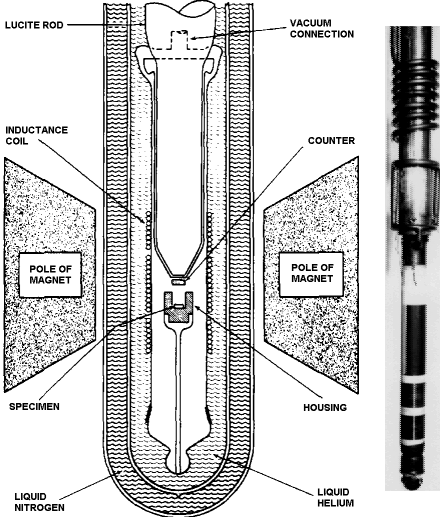
\includegraphics[width=\linewidth]{figs/setup.png}
%         \caption{Schematic illustration and photograph of the apparatus used in the Wu experiment \cite{NIST}.}
%         \label{fig:setup}
%     \end{subfigure}
%     \begin{subfigure}[b]{.39\linewidth}
%         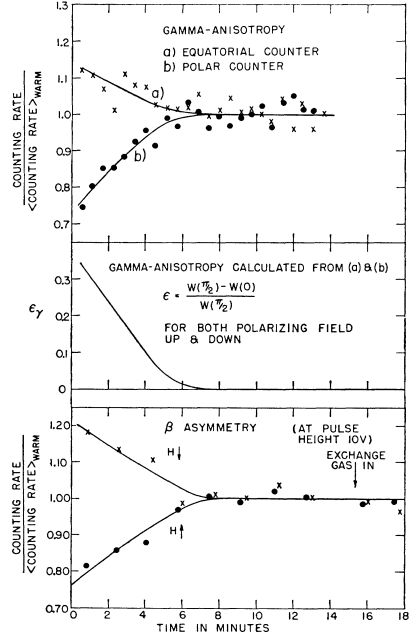
\includegraphics[width=\linewidth]{figs/resultsWu.png}
%         \caption{Measured results showing the gamma anisotropy and electron asymmetry for a polarizing magnetic field pointing up and down \cite{PhysRev.105.1413}.}
%         \label{fig:resultsWu}
%     \end{subfigure}
%     \label{fig:picsWu}
%     \caption{}
% \end{figure}